The wind powered car carrier (WPCC) has wind assisted ship propulsion (WASP) and can alter between a fully sailing mode, and a fully motoring mode -- and all in between. 
In this paper however, only the motoring mode is considered. Due to the WASP, the WPCC design differs a bit from conventional motoring cargo ship designs; The WPCC has two very large rudders -- the rudders are in fact two to three times as large as they would need to be for a conventional ships. The ship also has fins at the bilge, to generate extra lift while sailing, as seen on the scale model in \autoref{fig:WPCC}. 
%This figure also show two fans, that can be used to simulate wind forces, these were however not used in the manoeuvring tests of this paper. 
\autoref{tab:main_particulars} shows the main particulars of the scale model. 
\begin{figure}[h]
    \centering
    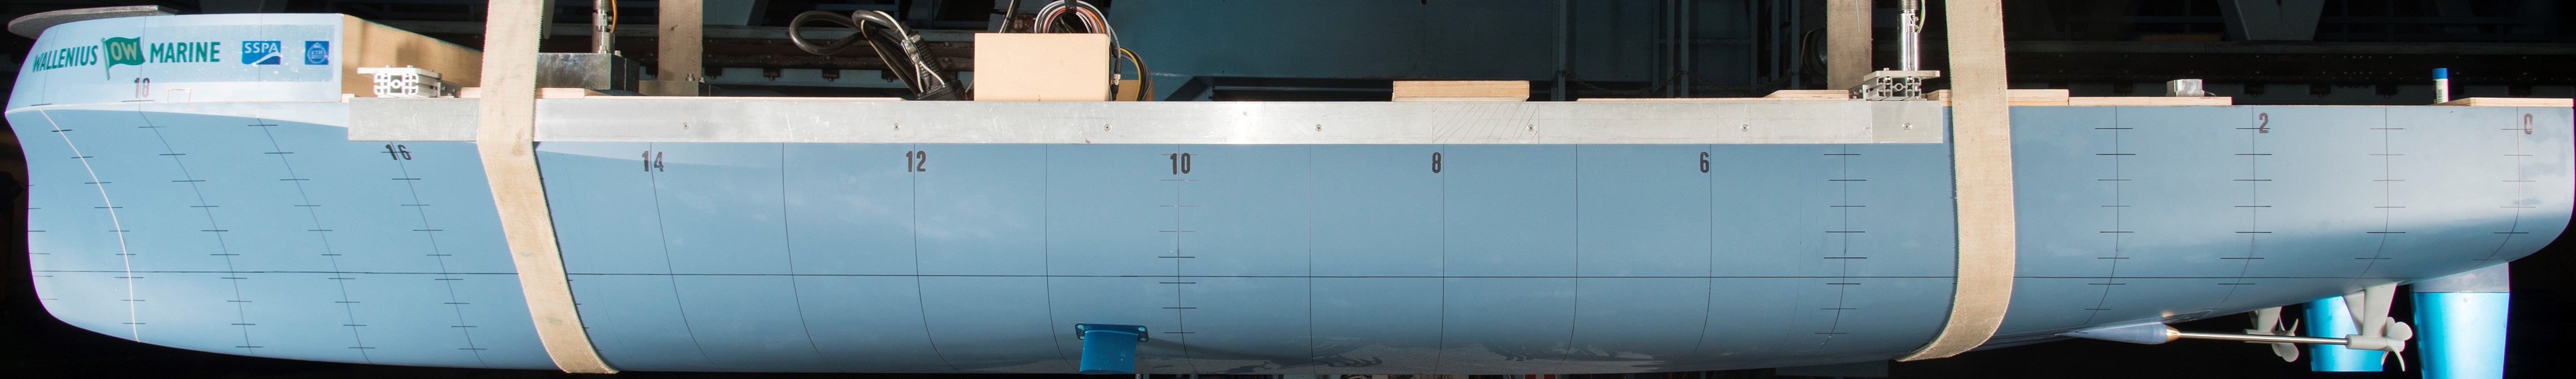
\includegraphics[width=\columnwidth]{figures/5m2.jpg}
    \caption{The scale model of the WPCC used in the model tests. Copyright RISE.}
    \label{fig:WPCC}
\end{figure}

Required input parameters for the semi-empirical rudder model are summarized in \autoref{tab:other_parameters}.
The rudder areas where obtained according to \autoref{fig:rudder_coverage}.   
Some manual tuning of the rudder drag was necessary, especially in the neutral rudder case, where the drag was increased almost 8 times as seen for $C_{D0tune}$. The rudder hull interaction coefficient $a_H$ was set to 0.12, reflecting that 12\% of the rudder force is generated on the ship hull.
Rudder angles above 15 degrees ($\delta_{lim}$) are assumed to be affected by the gap between rudder and rudder horn with an estimated strength $s$, which is based on experience from similar rudder arrangements.

The added mass coefficients are shown in \autoref{tab:added_masses}.
\begin{table}[h]
    \centering
    \caption{Main particulars (SI units) of WPCC scale model.}
    \label{tab:main_particulars}
    \pgfplotstabletypeset[col sep=comma, column type=r,
    columns/Parameter/.style={column type=l,string type},
    columns/Description/.style={column type=l,string type},
    columns/Value/.style={column type=r, column name=~},
    ]{tables/result_models.main_particulars.csv}
\end{table}